%---------------------------------------------------------------------- SLIDE -
\begin{frame}
\frametitle{Multi-valued abstractions: a gambling slot machine}
\begin{figure}[hbt]
\begin{center}
\fbox{
\begin{minipage}[b]{10cm}
{\tiny
\centerline{$m$: natural number;}
\centerline{$r_1:=?$; $r_2:=?$; $r_3:=?$;}

\vspace{4mm}
\parbox[t]{5cm}
{%\hspace{4mm}
$P_1::\left[\begin{array}{l}
              1.\ if\ m\%3=0\ \{\\
              2.\ \ \ random(r_1); \\
              3.\ \ \ if\ (r_1\neq ?\wedge r_2\neq ?\wedge r_3\neq ?) \\
              4.\ \ \ \ \ stop; \\
              5.\ \ \ if\ r_1=0 \\
              6.\ \ \ \ \ m:\ = m/3; \\
              7.\ \ \ else \\
              8.\ \ \ \ \ m:\ =m+2; \}
            \end{array}
      \right]$}
$\parallel$
{%\hspace{2mm}
$P_2::\left[\begin{array}{l}
              1.\ if\ m\%3=1\ \{ \\
              2.\ \ \ r_2:\ =r_1; \\
              3.\ \ \ if\ (r_1\neq ?\wedge r_2\neq ?\wedge r_3\neq ?) \\
              4.\ \ \ \ \ stop; \\
              5.\ \ \ m:\ = 2*m; \}
             \end{array}
      \right]$} \\
\begin{center}
$\parallel$ 
{$P_3::\left[\begin{array}{l}
              1.\ if\ m\%3=2\ \{^{DC}\\
              2.\ \ \ r_3:\ = r_2; \\
              3.\ \ \ if\ (r_1\neq ?\wedge r_2\neq ?\wedge r_3\neq ?) \\
              4.\ \ \ \ \ stop; \\              
              5.\ \ \ m:\ = 2*m-1; \}^{DC}                        
              \end{array}
      \right]$}
\end{center}
}
\end{minipage}
}
\end{center}
\end{figure}

\vspace{-1.5mm}
\begin{figure}[t]
		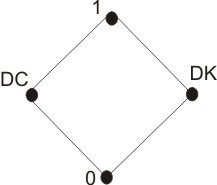
\includegraphics{figures/LatEx.jpg}
\end{figure}

\vspace{-1mm}
\begin{itemize}
\item \alert{$DC$ (don't care)}: values controlled by the environment 
\item \alert{$DK$ (don't know)}: values controlled by the system but not yet 
decided
\end{itemize}

\end{frame}

%---------------------------------------------------------------------- SLIDE -
\begin{frame}
\frametitle{Multi-valued abstractions: a gambling slot machine}
\begin{figure}[hbt]
\begin{center}
\fbox{
\begin{minipage}[b]{10cm}
{\tiny
\centerline{$m$: natural number;}
\centerline{$r_1:=?$; $r_2:=?$; $r_3:=?$;}

\vspace{4mm}
\parbox[t]{5cm}
{%\hspace{4mm}
$P_1::\left[\begin{array}{l}
              1.\ if\ m\%3=0\ \{\\
              2.\ \ \ random(r_1); \\
              3.\ \ \ if\ (r_1\neq ?\wedge r_2\neq ?\wedge r_3\neq ?) \\
              4.\ \ \ \ \ stop; \\
              5.\ \ \ if\ r_1=0 \\
              6.\ \ \ \ \ m:\ = m/3; \\
              7.\ \ \ else \\
              8.\ \ \ \ \ m:\ =m+2; \}
            \end{array}
      \right]$}
$\parallel$
{%\hspace{2mm}
$P_2::\left[\begin{array}{l}
              1.\ if\ m\%3=1\ \{ \\
              2.\ \ \ r_2:\ =r_1; \\
              3.\ \ \ if\ (r_1\neq ?\wedge r_2\neq ?\wedge r_3\neq ?) \\
              4.\ \ \ \ \ stop; \\
              5.\ \ \ m:\ = 2*m; \}
             \end{array}
      \right]$} \\
\begin{center}
$\parallel$ 
{$P_3::\left[\begin{array}{l}
              1.\ if\ m\%3=2\ \{^{DC}\\
              2.\ \ \ r_3:\ = r_2; \\
              3.\ \ \ if\ (r_1\neq ?\wedge r_2\neq ?\wedge r_3\neq ?) \\
              4.\ \ \ \ \ stop; \\              
              5.\ \ \ m:\ = 2*m-1; \}^{DC}                        
              \end{array}
      \right]$}
\end{center}
}
\end{minipage}
}
\end{center}
\end{figure}

\begin{itemize}
\item when the player pulls the handle, a random number $m$ 
is generated and then, each value of the reel on the pay line 
is determined by the values of $r_1$, $r_2$, and $r_3$
\item we suppose that the third reel has a malfunction:
the transitions of $P_3$ have the truth value $DC$
\item the player wins if $r_1=r_2=r_3=0$
\end{itemize}
\end{frame}

%---------------------------------------------------------------------- SLIDE -
\begin{frame}
\frametitle{Multi-valued abstractions: a gambling slot machine}
\begin{figure}[hbt]
\begin{center}
\fbox{
\begin{minipage}[b]{10cm}
{\tiny
\centerline{$m$: natural number;}
\centerline{$r_1:=?$; $r_2:=?$; $r_3:=?$;}

\vspace{4mm}
\parbox[t]{5cm}
{%\hspace{4mm}
$P_1::\left[\begin{array}{l}
              1.\ if\ m\%3=0\ \{\\
              2.\ \ \ random(r_1); \\
              3.\ \ \ if\ (r_1\neq ?\wedge r_2\neq ?\wedge r_3\neq ?) \\
              4.\ \ \ \ \ stop; \\
              5.\ \ \ if\ r_1=0 \\
              6.\ \ \ \ \ m:\ = m/3; \\
              7.\ \ \ else \\
              8.\ \ \ \ \ m:\ =m+2; \}
            \end{array}
      \right]$}
$\parallel$
{%\hspace{2mm}
$P_2::\left[\begin{array}{l}
              1.\ if\ m\%3=1\ \{ \\
              2.\ \ \ r_2:\ =r_1; \\
              3.\ \ \ if\ (r_1\neq ?\wedge r_2\neq ?\wedge r_3\neq ?) \\
              4.\ \ \ \ \ stop; \\
              5.\ \ \ m:\ = 2*m; \}
             \end{array}
      \right]$} \\
\begin{center}
$\parallel$ 
{$P_3::\left[\begin{array}{l}
              1.\ if\ m\%3=2\ \{^{DC}\\
              2.\ \ \ r_3:\ = r_2; \\
              3.\ \ \ if\ (r_1\neq ?\wedge r_2\neq ?\wedge r_3\neq ?) \\
              4.\ \ \ \ \ stop; \\              
              5.\ \ \ m:\ = 2*m-1; \}^{DC}                        
              \end{array}
      \right]$}
\end{center}
}
\end{minipage}
}
\end{center}
\end{figure}

\vspace{-1.5mm}
\begin{figure}[t]
		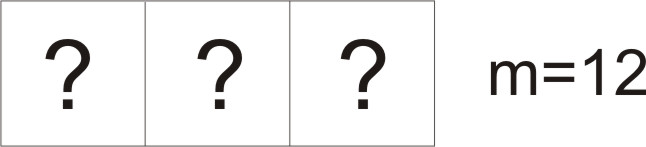
\includegraphics{figures/SlotMach1.jpg}
\end{figure}
\end{frame}


%---------------------------------------------------------------------- SLIDE -
\begin{frame}
\frametitle{Multi-valued abstractions: a gambling slot machine}
\begin{figure}[hbt]
\begin{center}
\fbox{
\begin{minipage}[b]{10cm}
{\tiny
\centerline{$m$: natural number;}
\centerline{$r_1:=?$; $r_2:=?$; $r_3:=?$;}

\vspace{4mm}
\parbox[t]{5cm}
{%\hspace{4mm}
$P_1::\left[\begin{array}{l}
              1.\ if\ m\%3=0\ \{\\
              2.\ \ \ random(r_1); \\
              3.\ \ \ if\ (r_1\neq ?\wedge r_2\neq ?\wedge r_3\neq ?) \\
              4.\ \ \ \ \ stop; \\
              5.\ \ \ if\ r_1=0 \\
              6.\ \ \ \ \ m:\ = m/3; \\
              7.\ \ \ else \\
              8.\ \ \ \ \ m:\ =m+2; \}
            \end{array}
      \right]$}
$\parallel$
{%\hspace{2mm}
$P_2::\left[\begin{array}{l}
              1.\ if\ m\%3=1\ \{ \\
              2.\ \ \ r_2:\ =r_1; \\
              3.\ \ \ if\ (r_1\neq ?\wedge r_2\neq ?\wedge r_3\neq ?) \\
              4.\ \ \ \ \ stop; \\
              5.\ \ \ m:\ = 2*m; \}
             \end{array}
      \right]$} \\
\begin{center}
$\parallel$ 
{$P_3::\left[\begin{array}{l}
              1.\ if\ m\%3=2\ \{^{DC}\\
              2.\ \ \ r_3:\ = r_2; \\
              3.\ \ \ if\ (r_1\neq ?\wedge r_2\neq ?\wedge r_3\neq ?) \\
              4.\ \ \ \ \ stop; \\              
              5.\ \ \ m:\ = 2*m-1; \}^{DC}                        
              \end{array}
      \right]$}
\end{center}
}
\end{minipage}
}
\end{center}
\end{figure}

\vspace{-1.5mm}
\begin{figure}[t]
		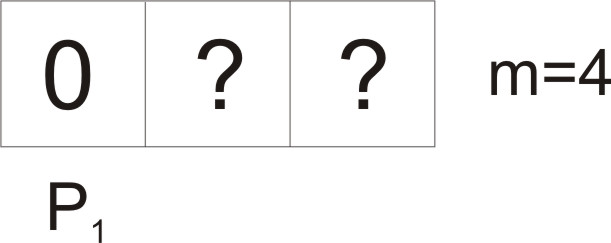
\includegraphics{figures/SlotMach2.jpg}
\end{figure}
\end{frame}

%---------------------------------------------------------------------- SLIDE -
\begin{frame}
\frametitle{Multi-valued abstractions: a gambling slot machine}
\begin{figure}[hbt]
\begin{center}
\fbox{
\begin{minipage}[b]{10cm}
{\tiny
\centerline{$m$: natural number;}
\centerline{$r_1:=?$; $r_2:=?$; $r_3:=?$;}

\vspace{4mm}
\parbox[t]{5cm}
{%\hspace{4mm}
$P_1::\left[\begin{array}{l}
              1.\ if\ m\%3=0\ \{\\
              2.\ \ \ random(r_1); \\
              3.\ \ \ if\ (r_1\neq ?\wedge r_2\neq ?\wedge r_3\neq ?) \\
              4.\ \ \ \ \ stop; \\
              5.\ \ \ if\ r_1=0 \\
              6.\ \ \ \ \ m:\ = m/3; \\
              7.\ \ \ else \\
              8.\ \ \ \ \ m:\ =m+2; \}
            \end{array}
      \right]$}
$\parallel$
{%\hspace{2mm}
$P_2::\left[\begin{array}{l}
              1.\ if\ m\%3=1\ \{ \\
              2.\ \ \ r_2:\ =r_1; \\
              3.\ \ \ if\ (r_1\neq ?\wedge r_2\neq ?\wedge r_3\neq ?) \\
              4.\ \ \ \ \ stop; \\
              5.\ \ \ m:\ = 2*m; \}
             \end{array}
      \right]$} \\
\begin{center}
$\parallel$ 
{$P_3::\left[\begin{array}{l}
              1.\ if\ m\%3=2\ \{^{DC}\\
              2.\ \ \ r_3:\ = r_2; \\
              3.\ \ \ if\ (r_1\neq ?\wedge r_2\neq ?\wedge r_3\neq ?) \\
              4.\ \ \ \ \ stop; \\              
              5.\ \ \ m:\ = 2*m-1; \}^{DC}                        
              \end{array}
      \right]$}
\end{center}
}
\end{minipage}
}
\end{center}
\end{figure}

\vspace{-1.5mm}
\begin{figure}[t]
		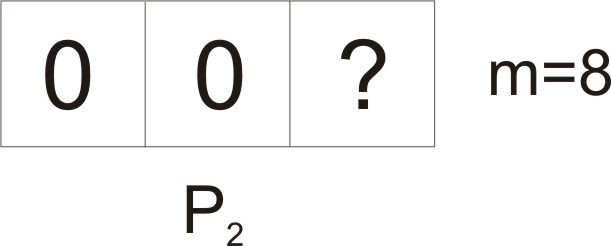
\includegraphics{figures/SlotMach3.jpg}
\end{figure}
\end{frame}

%---------------------------------------------------------------------- SLIDE -
\begin{frame}
\frametitle{Multi-valued abstractions: a gambling slot machine}
\begin{figure}[hbt]
\begin{center}
\fbox{
\begin{minipage}[b]{10cm}
{\tiny
\centerline{$m$: natural number;}
\centerline{$r_1:=?$; $r_2:=?$; $r_3:=?$;}

\vspace{4mm}
\parbox[t]{5cm}
{%\hspace{4mm}
$P_1::\left[\begin{array}{l}
              1.\ if\ m\%3=0\ \{\\
              2.\ \ \ random(r_1); \\
              3.\ \ \ if\ (r_1\neq ?\wedge r_2\neq ?\wedge r_3\neq ?) \\
              4.\ \ \ \ \ stop; \\
              5.\ \ \ if\ r_1=0 \\
              6.\ \ \ \ \ m:\ = m/3; \\
              7.\ \ \ else \\
              8.\ \ \ \ \ m:\ =m+2; \}
            \end{array}
      \right]$}
$\parallel$
{%\hspace{2mm}
$P_2::\left[\begin{array}{l}
              1.\ if\ m\%3=1\ \{ \\
              2.\ \ \ r_2:\ =r_1; \\
              3.\ \ \ if\ (r_1\neq ?\wedge r_2\neq ?\wedge r_3\neq ?) \\
              4.\ \ \ \ \ stop; \\
              5.\ \ \ m:\ = 2*m; \}
             \end{array}
      \right]$} \\
\begin{center}
$\parallel$ 
{$P_3::\left[\begin{array}{l}
              1.\ if\ m\%3=2\ \{^{DC}\\
              2.\ \ \ r_3:\ = r_2; \\
              3.\ \ \ if\ (r_1\neq ?\wedge r_2\neq ?\wedge r_3\neq ?) \\
              4.\ \ \ \ \ stop; \\              
              5.\ \ \ m:\ = 2*m-1; \}^{DC}                        
              \end{array}
      \right]$}
\end{center}
}
\end{minipage}
}
\end{center}
\end{figure}

\vspace{-1.5mm}
\begin{figure}[t]
		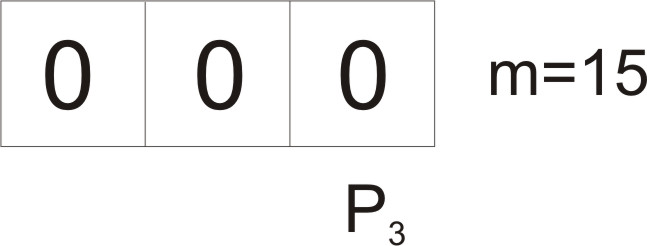
\includegraphics{figures/SlotMach4.jpg}
\end{figure}
\end{frame}

%---------------------------------------------------------------------- SLIDE -
\begin{frame}
\frametitle{Multi-valued abstractions: a gambling slot machine}
\begin{figure}[hbt]
\begin{center}
\fbox{
\begin{minipage}[b]{10cm}
{\tiny
\centerline{$m$: natural number;}
\centerline{$r_1:=?$; $r_2:=?$; $r_3:=?$;}

\vspace{4mm}
\parbox[t]{5cm}
{%\hspace{4mm}
$P_1::\left[\begin{array}{l}
              1.\ if\ m\%3=0\ \{\\
              2.\ \ \ random(r_1); \\
              3.\ \ \ if\ (r_1\neq ?\wedge r_2\neq ?\wedge r_3\neq ?) \\
              4.\ \ \ \ \ stop; \\
              5.\ \ \ if\ r_1=0 \\
              6.\ \ \ \ \ m:\ = m/3; \\
              7.\ \ \ else \\
              8.\ \ \ \ \ m:\ =m+2; \}
            \end{array}
      \right]$}
$\parallel$
{%\hspace{2mm}
$P_2::\left[\begin{array}{l}
              1.\ if\ m\%3=1\ \{ \\
              2.\ \ \ r_2:\ =r_1; \\
              3.\ \ \ if\ (r_1\neq ?\wedge r_2\neq ?\wedge r_3\neq ?) \\
              4.\ \ \ \ \ stop; \\
              5.\ \ \ m:\ = 2*m; \}
             \end{array}
      \right]$} \\
\begin{center}
$\parallel$ 
{$P_3::\left[\begin{array}{l}
              1.\ if\ m\%3=2\ \{^{DC}\\
              2.\ \ \ r_3:\ = r_2; \\
              3.\ \ \ if\ (r_1\neq ?\wedge r_2\neq ?\wedge r_3\neq ?) \\
              4.\ \ \ \ \ stop; \\              
              5.\ \ \ m:\ = 2*m-1; \}^{DC}                        
              \end{array}
      \right]$}
\end{center}
}
\end{minipage}
}
\end{center}
\end{figure}

\vspace{-1.5mm}
\begin{figure}[t]
		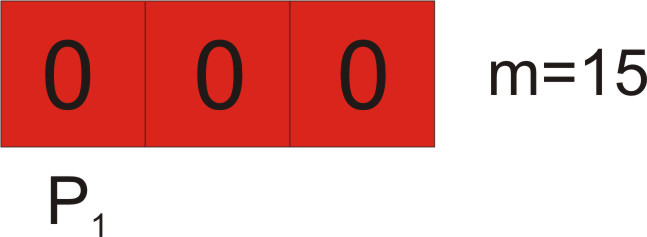
\includegraphics{figures/SlotMach5.jpg}
\end{figure}
\end{frame}

%---------------------------------------------------------------------- SLIDE -
\begin{frame}
\frametitle{Multi-valued abstractions: a gambling slot machine}
\begin{figure}[hbt]
\begin{center}
\fbox{
\begin{minipage}[b]{10cm}
{\tiny
\centerline{$m$: natural number;}
\centerline{$r_1:=?$; $r_2:=?$; $r_3:=?$;}

\vspace{4mm}
\parbox[t]{5cm}
{%\hspace{4mm}
$P_1::\left[\begin{array}{l}
              1.\ if\ m\%3=0\ \{\\
              2.\ \ \ random(r_1); \\
              3.\ \ \ if\ (r_1\neq ?\wedge r_2\neq ?\wedge r_3\neq ?) \\
              4.\ \ \ \ \ stop; \\
              5.\ \ \ if\ r_1=0 \\
              6.\ \ \ \ \ m:\ = m/3; \\
              7.\ \ \ else \\
              8.\ \ \ \ \ m:\ =m+2; \}
            \end{array}
      \right]$}
$\parallel$
{%\hspace{2mm}
$P_2::\left[\begin{array}{l}
              1.\ if\ m\%3=1\ \{ \\
              2.\ \ \ r_2:\ =r_1; \\
              3.\ \ \ if\ (r_1\neq ?\wedge r_2\neq ?\wedge r_3\neq ?) \\
              4.\ \ \ \ \ stop; \\
              5.\ \ \ m:\ = 2*m; \}
             \end{array}
      \right]$} \\
\begin{center}
$\parallel$ 
{$P_3::\left[\begin{array}{l}
              1.\ if\ m\%3=2\ \{^{DC}\\
              2.\ \ \ r_3:\ = r_2; \\
              3.\ \ \ if\ (r_1\neq ?\wedge r_2\neq ?\wedge r_3\neq ?) \\
              4.\ \ \ \ \ stop; \\              
              5.\ \ \ m:\ = 2*m-1; \}^{DC}                        
              \end{array}
      \right]$}
\end{center}
}
\end{minipage}
}
\end{center}
\end{figure}

\begin{itemize}
	\item $M=(Q,R,L)$ models this system, where:
%	 by \alert{a multi-valued Kripke structure } 
%over a set of atomic propositions $AP=\blue{\{win,undef\}}$, where:
	\begin{itemize}
	\setlength\itemsep{1ex}
   \item $Q=\{\alert{(m,r_1,r_2,r_3)}|m\in\bN\mbox{ and }r_1,r_2,r_3\in\bN\cup\{?\}\}$;
   \item $R$ is defined according to the program above and $D=\{DC,DK,1\}$;
   \item $L$ labels the states by \blue{$win$} and \blue{$undef$} as follows:
       \begin{itemize}
           \item \blue{$win$} is 1 in states with $r_1=r_2=r_3=0$, $DK$ in states
           with at least one $r_i=?$, and 0, otherwise.
           \item \blue{$undef$} is 1 in states for which there exists an $r_i=?$,
           and 0, otherwise. 
       \end{itemize}
	\end{itemize}
\end{itemize}
\end{frame}

%---------------------------------------------------------------------- SLIDE -
\begin{frame}
\frametitle{Multi-valued abstractions: a gambling slot machine}

Goal: check the $\forall CTL^*_+$ formula 
\alert{$\phi=\forall\,\bG\,(undef\vee win)$}

%\vspace{3mm}
\begin{itemize}
	\item define an abstraction of $M$ by:
	\begin{itemize}
		\item \alert{$(m,r_1,r_2,r_3)\ \rho\ (m',r_1',r_2',r_3')$} iff:
		\[
		m\%3=m'\%3\mbox{ and }\bigwedge_{1\leq i\leq 3}(r_i=r_i'=?\vee 
		r_i=r_i'=0\vee (r_i>0\wedge r_i'>0))
		\]
		\item 
		\begin{tabular}[t]{l|c|c|c|c}
		Truth values\ \ & $0$ & $DC$ & $DK$ & $1$ \\ [1mm]\hline
		\alert{policy $\alpha_R$} & $\forall$ & $\exists$ & 
		        $\exists^{\{0,DK,1\}}$ & $\exists^{\{0,1\}}$ \\ [1mm]\hline
		\alert{policy $\alpha_L$} & $\exists^{\{0,DC,1\}}$ & 
		        $\exists^{\{DC,1\}}$ & $\exists^{\{0,DK,1\}}$ & $\forall$ 
		\end{tabular}
	\end{itemize}
\end{itemize}

\vspace{-3mm}
\begin{figure}[t]
	\centering
		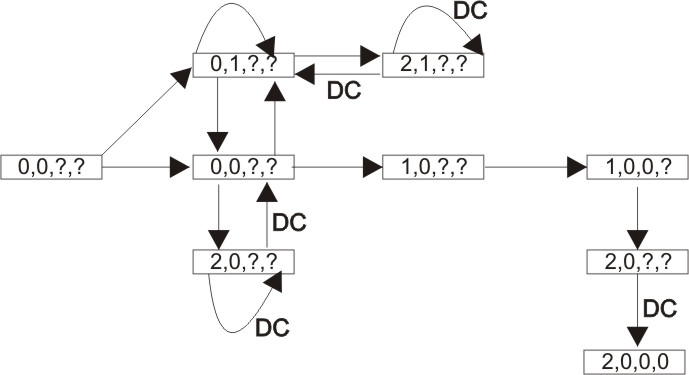
\includegraphics{figures/abstraction.jpg}
%	\caption{The $(\alpha_R,\alpha_L)$-abstraction of $M$ by $\rho$}
%	\label{fabs}
\end{figure}
\end{frame}

%---------------------------------------------------------------------- SLIDE -
\begin{frame}
\frametitle{Multi-valued abstractions: a gambling slot machine}

Property transfer:
\vspace{2mm}
\begin{itemize}
\setlength\itemsep{2ex}
\item the truth value of $\phi$ in any state of the abstract system 
is $\geq DC$
\item by the previous preservation result, we obtain
that \alert{the truth value of $\phi$ in any state of the concrete system 
is $\geq DC$}
\end{itemize}
\end{frame}